% % % % % % % % % % % % % % % % % % % % % % % % % % % % % % % % % %
\documentclass[11pt, journal]{IEEEtran}

% packages
\usepackage{amsmath,amssymb,amsthm,stmaryrd}
\usepackage{amsbsy}
\usepackage{balance}
\usepackage{booktabs}
\usepackage{bold-extra}
\usepackage{bigstrut}
\newtheorem{corollary}{Corollary}
\newtheorem{convention}{Convention}
\usepackage[outerbars,color]{changebar}
%\usepackage{float}
\usepackage{graphicx}
\usepackage{ifthen}
\usepackage{multirow}
\usepackage{microtype}
\usepackage{needspace}
\usepackage{rotating}
\usepackage{subfig}
\usepackage{verbatim}
\usepackage{xspace}
%\usepackage[table]{xcolor}
\usepackage[table,usenames,dvipsnames]{xcolor}
%\usepackage[normalem]{ulem} %emphasize still italic
\usepackage{url}
\usepackage{tabularx}
\usepackage{cite}


\newcommand\set[1]{\{#1\}}
\newcommand\inv[1]{#1^{-1}}

%\newtheorem{theorem}{Theorem}
\newtheorem{definition}{Definition}
%\newtheorem{example}{Example}
%


%\usepackage[utf8]{inputenc} 
%\usepackage[T1]{fontenc}
%\usepackage[upright]{fourier} 
%\usepackage[usenames,dvipsnames]{xcolor}
%\usepackage{tkz-kiviat,numprint,fullpage} 
%\usepackage{tkz-kiviat} 
%\listfiles


% constants
\newcommand{\Title}{Survey on intra-actor Parallelism in the Actor Model}
\newcommand{\TitleShort}{Intra actor Parallelism in the Actor Model}
\newcommand{\Authors}{Michael R\"ufenacht}
\newcommand{\AuthorsShort}{M. R\"ufenacht}

\newcounter{qcounter}

% references
\usepackage[colorlinks,
	bookmarks=false %REMOVE BOOKMARKS
	]{hyperref}
\usepackage[all]{hypcap}
\setcounter{tocdepth}{2}
\hypersetup{
	colorlinks=true,
	urlcolor=black,
	linkcolor=black,
	citecolor=black,
	plainpages=false,
	bookmarksopen=true,
	pdfauthor={\Authors}%,pdftitle={\Title}
}
\def\UrlFont{\footnotesize\ttfamily}

% source code
\usepackage{xcolor}
\usepackage{textcomp}
\usepackage{listings}
\definecolor{source}{gray}{0.9}
\lstset{
	language={},
	% characters
	tabsize=2,
	upquote=true,
	escapechar={!},
	keepspaces=true,
	breaklines=true,
	alsoletter={:},
	breakautoindent=true,
	columns=fullflexible,
	showstringspaces=false,
	basicstyle=\footnotesize\ttfamily,
	% background
	frame=single,
    framerule=0pt,
	backgroundcolor=\color{source},
	% numbering
	numbersep=5pt,
	numberstyle=\tiny,
	numberfirstline=true,
	% captioning
	captionpos=b,
	numberbychapter=false,
	% formatting (html)
	moredelim=[is][\textbf]{<b>}{</b>},
	moredelim=[is][\textit]{<i>}{</i>},
	moredelim=[is][\uline]{<u>}{</u>}}
\newcommand{\ct}{\lstinline[backgroundcolor=\color{white},basicstyle=\footnotesize\ttfamily]}
\newcommand{\lct}[1]{{\small\tt #1}}
\lstnewenvironment{code}[1][]%
  {\minipage{\linewidth}\lstset{#1}}
  {\endminipage}

% tikz
% \usepackage{tikz}
% \usetikzlibrary{fit}
% \usetikzlibrary{arrows}
% \usetikzlibrary{external}
% \usetikzlibrary{positioning}
% \usetikzlibrary{backgrounds}
% \usetikzlibrary{shapes.multipart}
% \usetikzlibrary{shapes.geometric}

% references
\newcommand{\tabref}[1]{\hyperref[{tab:#1}]{Table~\ref*{tab:#1}}}
\newcommand{\figref}[1]{\hyperref[{fig:#1}]{Figure~\ref*{fig:#1}}}
\newcommand{\secref}[1]{\hyperref[{sec:#1}]{Section~\ref*{sec:#1}}}
\newcommand{\lstref}[1]{\hyperref[{lst:#1}]{Listing~\ref*{lst:#1}}}
\newcommand{\defref}[1]{\hyperref[{def:#1}]{Definition~\ref*{def:#1}}}

%%%%%%%%%%%%%%%%%%%%%%%%%%%%%%%
%Removing space after the caption of floating elements
%\addtolength{\belowcaptionskip}{-4mm}
%\addtolength{\textfloatsep}{-7mm}


%%%%%%%%%%%%%%%%%%%%%%%%%%%%%%%%%%%%%%%%%%%%%%%
% Markup macros for proof-reading
\usepackage[normalem]{ulem} % for \sout
\usepackage{xcolor}
\newcommand{\ra}{$\rightarrow$}
\newcommand{\ugh}[1]{\textcolor{red}{\uwave{#1}}} % please rephrase
\newcommand{\ins}[1]{\textcolor{blue}{\uline{#1}}} % please insert
\newcommand{\del}[1]{\textcolor{red}{\sout{#1}}} % please delete
\newcommand{\chg}[2]{\textcolor{red}{\sout{#1}}{\ra}\textcolor{blue}{\uline{#2}}} % please change
\newcommand{\mlchg}[2]{\textcolor{gray}{\sout{#1}}{\ra}\textcolor{olive}{\uline{#2}}} % please change

% graphics: \fig{position}{relative-width}{filename}{caption}
%\newcommand{\lessSpace}{\vspace{-1em}}
%\DeclareGraphicsExtensions{.pdf,.png}
%\graphicspath{{figures/}}
%\newcommand{\fig}[4]{
%	\begin{figure}[#1]
%		\centering
%		\includegraphics[width=#2\textwidth]{images/#3}
%		\lessSpace
%		\caption{\label{fig:#3}#4}
%	\end{figure}}

% abbreviations
\newcommand{\ie}{\emph{i.e.,}\xspace}
\newcommand{\eg}{\emph{e.g.,}\xspace}
\newcommand{\etc}{\emph{etc.}\xspace}
\newcommand{\etal}{\emph{et al.}\xspace}

% commands
\newcommand{\n}{$\cdot$}
\newcommand{\y}{\checkmark}
\newcommand{\subscript}[1]{$_{\textrm{\footnotesize{#1}}}$}
\newcommand{\superscript}[1]{$^{\textrm{\footnotesize{#1}}}$}
\newcommand{\vertical}[1]{\raisebox{-4em}{\begin{sideways}{#1}\end{sideways}}}

% notes
%\newcommand\aanote[1]{\marginpar{\tiny [#1]}}
%\newcommand\aanote[1]{[{\bf aa:}{\footnotesize #1 }]}
%\newcommand\ml[1]{[{\bf ml:}{\footnotesize #1 }]}

% Put edit comments in a really ugly standout display
\usepackage{amssymb}

\newboolean{showcomments}
\setboolean{showcomments}{true}
%\setboolean{showcomments}{false}

\newcommand{\yellowbox}[1]{\fcolorbox{gray}{yellow}{\bfseries\sffamily\scriptsize#1}}
\newcommand{\triangles}[1]{{\sf\small$\blacktriangleright$\textit{#1}$\blacktriangleleft$}}
\ifthenelse{\boolean{showcomments}}
{\newcommand{\nbc}[3]{
 {\colorbox{#3}{\bfseries\sffamily\scriptsize\textcolor{white}{#1}}}
 {\textcolor{#3}{\sf\small$\blacktriangleright$\textit{#2}$\blacktriangleleft$}}}
 \newcommand{\version}{\emph{\scriptsize\id}}}
{\newcommand{\nbc}[3]{}
 \renewcommand{\ugh}[1]{#1} % please rephrase
 \renewcommand{\ins}[1]{#1} % please insert
 \renewcommand{\del}[1]{#1} % please delete
 \renewcommand{\chg}[2]{#2} % please change
 \newcommand{\version}{}}
\newcommand{\nb}[2]{\nbc{#1}{#2}{orange}}
\newcommand{\here}{\yellowbox{$\Rightarrow$ CONTINUE HERE $\Leftarrow$}}
\newcommand\rev[2]{\nb{TODO (rev #1)}{#2}} % reviewer comments
\newcommand\fix[1]{\nb{FIX}{#1}}
\newcommand\todo[1]{\nb{TO DO}{#1}}
\newcommand\jr[1]{\nbc{JR}{#1}{orange}}
\newcommand\on[1]{\nbc{ON}{#1}{orange}}
\newcommand\fp[1]{\nbc{FP}{#1}{purple}}
\newcommand\mr[1]{\nbc{MR}{#1}{olive}}
\newcommand\yh[1]{\nbc{YH}{#1}{red}}

\renewcommand{\labelitemi}{$\bullet$}
\definecolor{myColor}{rgb}{0.9,0.9,0.9}



%You can now add footnotes in your document, and remember a reference to them with, e.g.,
%\footnoteremember{myfootnote}{This is my footnote}
%and then refer to this footnote again with
%\footnoterecall{myfootnote}.
\newcommand{\footnoteremember}[2]{
  \footnote{#2}
  \newcounter{#1}
  \setcounter{#1}{\value{footnote}}
}
\newcommand{\footnoterecall}[1]{
  \footnotemark[\value{#1}]
}
\newcommand{\X}{$\times$ }
\newcommand{\Bull}{$\bullet$ }

%Environments
\newenvironment{cb}{\cbstart\cbcolor{blue}\color{gray}}{\cbend}
\newenvironment{cml}{\cbstart\cbcolor{red}\color{black}}{\cbend}


%:Math variable names
\newcommand{\rel}{\mathit{REL}}
\newcommand{\has}{\mathit{HAS}}
\newcommand{\use}{\mathit{USE}}
\newcommand{\cnc}{\mathit{CNC}}

\newcommand{\CLS}{\mathit{CLS}}
\newcommand{\cls}{\mathit{cls}}
\newcommand{\ATT}{\mathit{ATT}}
\newcommand{\MET}{\mathit{MET}}
\newcommand{\TBL}{\mathit{TBL}}
\newcommand{\tbl}{\mathit{t}}

\newcommand{\REF}{\mathit{REF}}
\newcommand{\MAP}{\mathit{MAP}}
\newcommand{\ACC}{\mathit{ACC}}



\newcommand{\scr}{\mathit{s}}
\newcommand{\SCR}{\mathit{S}}

% tikz
%\usepackage{tikz}
%\usetikzlibrary{matrix}
%\usetikzlibrary{arrows}
%\usetikzlibrary{external}
%\usetikzlibrary{positioning}
%\usetikzlibrary{shapes.multipart}
%
%\tikzset{
%	every picture/.style={semithick, font=\scriptsize},
%	every text node part/.style={align=center}}

% D O C U M E N T
% % % % % % % % % % % % % % % % % % % % % % % % % % % % % % % % % %
\begin{document}
% avoid repeating names to be replaced by ----
\bstctlcite{IEEEexample:BSTcontrol}

% T I T L E
% % % % % % % % % % % % % % % % % % % % % % % % % % % % % % % % % %
\title{\Title}
\thispagestyle{empty}
\author{
	\IEEEauthorblockN{\Authors}\\				
	\IEEEauthorblockA{
		\texttt{m.ruefenacht@students.unibe.ch}\\
		Joint Master in Computer Science\\
		Workshop 2013\\
		University of Neuch\^atel, Switzerland\\
	}
}
		
\maketitle
%\thanks{}

%\begin{comment}
%keywords:
%%Domain-based coupling
%%Architectural dependencies
%%Database dependencies
%%Source code analysis
%%Program comprehension
%\end{comment}

%\vspace{-15pt}

% A B S T R A C T
% % % % % % % % % % % % % % % % % % % % % % % % % % % % % % % % % %
\begin{abstract}
The paradigm shift from centralized and serial to distributed and concurrent computing, introduced the need for models that fulfill the inherently concurrent nature of such systems. One example of a model, which recently regained researcher's attention, is the Actor Model. Concurrency issues in thread-based systems are explicitly handled by the application layer what appears to be complex and error prone. The Actor Model, in comparison, implicitly avoids possibly arising concurrency issues such as race conditions. Its strict semantics introduce strong guarantees, but also limit the scalability of actor-based systems. One of the Actor Model's main drawbacks is the difficulty to exploit intra-actor parallelism when processing incoming messages. This paper presents a survey of the model itself and approaches targeted at enriching the Actor Model with parallel processing of messages and the concurrent execution of code sections within actors.
\end{abstract}

% I N T R O D U C T I O N
% % % % % % % % % % % % % % % % % % % % % % % % % % % % % % % % % %
\section{Introduction}\label{sec:introduction}
Created by Carl Hewitt et al.~\cite{Hewitt:1973:UMA:1624775.1624804} in the early seventies, the Actor Model was further formalized and theoretically refined in publications from Grief~\cite{Grief:1975:SCP:888942} Hewitt et al.~\cite{Hewi77a} or Agha~\cite{Agha:1985:AMC:912083} just to name a few.
The widespread use of multi-core architectures and distributed computing introduced the need for adequate models to safely exploit concurrency~\cite{Sutter:2005:SCR:1095408.1095421}. The Actor Model fits the characteristics and requirements of parallel and concurrent systems by design and inherently avoids arising concurrency issues. The model and its entities underly strict data access and behavioral semantics. In contrast to thread-based environments, concurrency in the Actor Model is achieved by using asynchronous message passing.\\ 
Beside academic interests and the possibility of reasoning on its internal state, the Actor Model meanwhile was implemented in a number of languages\footnote{such as Erlang, Scala, AmbientTalk \dots} and integrated with frameworks, such as the Akka library\footnote{\url{http://akka.io/}}. Usual concurrency problems such as race conditions, deadlocks, starvation or liveness issues cannot occur in actor-based systems. Despite being beneficial in many aspects the aforementioned strong semantics constrain concurrency and therefore limit scalability. Attempts to exploit the full benefits of parallelism to improve scalability, rely on relaxations of the of the Actor Model and its semantics. To increase the level of abstraction, the approaches reviewed in the following sections, introduce appropriate mechanisms such as additional language constructs e.g. for convenient handling of synchronization. This survey presents two approaches which target at the improvement of scalability of the basic Actor Model by enabling parallel message processing.\\\\
{\bf\emph{Outline.}}
The paper starts with an overview of the main Actor Model characteristics in \secref{actor_model}. \secref{pam} explores the concept of Parallel Actor Monitors (PAM) which allow the injection of message schedulers into actors. In \secref{unifiedmodel}, I discuss the Unified Model (UM) which combines the Actor Model with the Async-Finish Model (AFM). \secref{comparison} briefly compares PAM to the UM and their capabilities to exploit intra-actor parallelism. \secref{conclusion} concludes before I briefly discuss the effectiveness of the presented concepts.\\

%  Actor Model
% % % % % % % % % % % % % % % % % % % % % % % % % % % % % % % % % %
\section{The Actor Model}\label{sec:actor_model}
In essence, the Actor Model consists of two concepts: the actor entities and asynchronous message passing. Actors (\cite{Hewitt:1973:UMA:1624775.1624804}) are self-contained (\cite{Agha:1990:COP:83880.84528}), strongly encapsulating entities. They can be composed to systems and communicate by asynchronous message passing \cite{Agha:1990:COP:83880.84528} under strong semantics as formalized by Agha~\cite{Agha:1990:SSA:648142.749964}, Clinger~\cite{Clinger:1981:FAS:889486} or Grief~\cite{Grief:1975:SCP:888942}.

\subsection{The actor}\label{subsec:actor}
Actors as the main entities of the Actor Model follow the \textit{'everything is an actor'} credo, similar to the \textit{'everything is an object'} paradigm. Actors have a restricted set of fundamental capabilities:

\begin{itemize}
	\item send a finite amount of messages to other actors
	\item receive a finite amount of messages from other actors
	\item spawn new actors
	\item change their internal state (become another actor)
\end{itemize}

One of actor's most important characteristics are also the Actor Model's strongest limitations: strong encapsulation and locality. An actor can be stateful but the Actor Model removes the feasibility to access another actor's internal state. Although an actor can expose information about its state by appropriate messages, there exists no shared mutable state. In general, actors can be viewed as black-boxes, having references to other actors instances only. This concept of strong encapsulation inherently creates mutual exclusion without synchronization and locking. As a consequence, an actor is constrained to send messages to already known addresses from incoming messages or spawned actors only, which is referred to as locality.

\subsection{Asynchronous message passing}\label{subsec:messagepassing}
Communication between actors is handled by asynchronous message passing. A message consists of an actor's address (or identifier), the return address and the data (sometimes referred to as \textit{message payload}). Depending on the Actor Model implementation, an actor determines appropriate behavior based on the type of the incoming message.\\

Actors store received messages in an unique storage facility known as a mailbox. The Actor Model ensures fairness by providing weak message delivery guarantees, meaning that every message gets eventually delivered. In Object-Oriented Programming the invocation of a method on an object can lock the invoking entity. The emission of messages in the Actor Model happens asynchronously and does not block the sender. The non blocking communication enables the actors to work in parallel and avoids locking of system resources~\cite{Karmani:2009:AFJ:1596655.1596658} (e.g. a system stack).

An actor is not required to process messages in any particular order (what Hewitt et al. refer to as \textit{particular order of events}~\cite{Hewi77a}). The absence of constraints on the order of message delivery corresponds to non-determinism, an essential property of parallel computing.
Nevertheless, an actor is only permitted to process one message at a time, a decision that was made upon the introduction of stateful actors~\cite{Yonezawa:1990:AOC:77683}. Allowing two messages to be processed in parallel leads to concurrent access to the internal state of the actors.
While this limitation guarantees the absence of deadlocks and data races, it puts a serious limitation on task level parallelism. 
Also, the absence of shared mutable state requires libraries implementing the Actor Model to support call-by-value semantics~\cite{Karmani:2009:AFJ:1596655.1596658} (i.e. which would avoid shared references).

\subsection{Parallel message processing and data partitioning}\label{subsec:messageprocessinganddatapartitioning}
As elaborated earlier, an actor is only allowed to process one message at a time which implies serial processing of the internal message queue. 

Nevertheless it is possible to establish a certain degree of parallelism by delegating parts of the computation to other actors, which would process them in parallel. An actor can therefore implement a \textit{divide-and-conquer} strategy and spawn new actors that compute partial results on a chunk of data. Scholliers et al.~\cite{Scholliers2010a} emphasize the resulting coupling between data and computation.\\
One strategy to enable the delegation of data-coupled tasks to new actors, is data partitioning \cite{Diaconescu02a}. An actor therefore is responsible to create data chunks (of incoming or contained data) and for provisioning them together with the necessary parameters to the spawned actors upon initialization. Since the Actor Model does not permit the parent actor and the spawned actors to have access to the same data, the parent actor has to release its lock on the partition or create a copy before passing it to the child. In this case Actor Model semantics can be fully preserved, but partitioning and copying of the data are expensive tasks and cause the majority of the mentioned overheads. Furthermore, executing global actions on the distributed data chunks are accompanied with a high degree of overhead associated with controlling and coordination. Examples of global actions are search operations over several actors or data manipulations, that require other actors to update their part of the data.

\subsection{Improvements}\label{subsec:improvements}
The Actor Model introduces several desirable characteristics one example being its abstraction of concurrency and strong guarantees for concurrent systems. As stated previously, these advantages introduce a trade-off between data-race-freedom and efficiency caused by the sequential message processing inside an actor. Attempts such as data partitioning to achieve the desired task level parallelism without violating the Actor Model, cause overheads~\cite{Scholliers2010a}. The following approaches try to establish other strategies to improve parallelism (and therefore introduce violations of the model and its semantics). 

\subsection{An example of message processing}\label{subsec:example}To demonstrate the differences and benefits the following approaches provide, we consider a contrived table actor. It stores an encapsulated, two dimensional data structure (a table), organized in indexed rows which are accessible via ID. The table actor acts as a read/write service for an arbitrary number of clients (similar to an indexed table in a relational database management system). The restriction to process one message at a time enforces the actor to subsequently execute both, the read and the write messages, under mutual exclusion. The resulting impossibility to exploit parallelism in the given scenario creates a bottleneck and hence limits scalability. \figref{serialprocessing}, provides an example of a message arrival sequence, comparing computation time (x-axis) to the progress in message queue processing (y-axis).

\begin{figure}[!htbp]
	\centering
	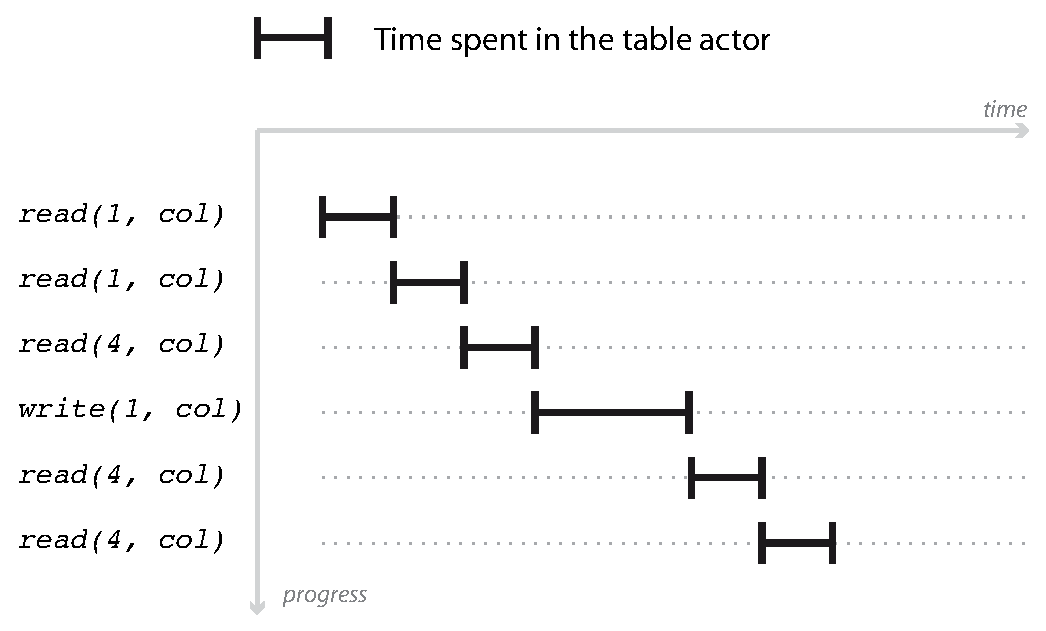
\includegraphics[width=\columnwidth]{figures/processing-01.eps}
	\begin{caption} {default serial execution of read and} write accesses to different rows (and columns)\label{fig:serialprocessing}\end{caption}
\end{figure}

Implementing a data partition strategy in this context is straightforward. The table actor spawns row actors and passes the corresponding data chunks to them. Hence, reads and writes to disjoint rows can be executed in parallel (the table actor still only processes one message at the time, by simply delegating the access), illustrated in \autoref{fig:partitionedprocessing}. The emerging overheads depend on the complexity and size of the underlying data structure. In addition, the partitioned processing causes a larger memory footprint and complicates global actions. A good example for such an operation would be searching, which would require consulting all rows (probably even locking them) and handle the join of the results (an issue that was also identified by Imam et al.~\cite{Imam:2012:ITP:2384616.2384671} and solved in their Unified Model implementation).
\begin{figure}[!htbp]
	\centering
	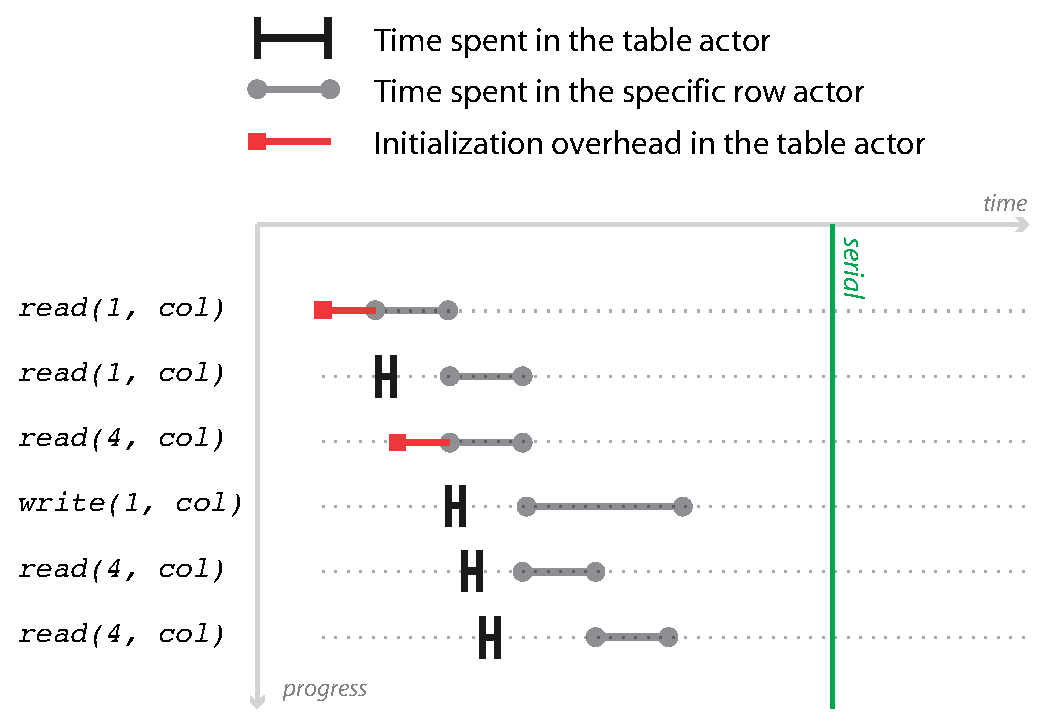
\includegraphics[width=\columnwidth]{figures/processing-02.eps}
	\begin{caption} {partially parallel execution} after data partitioning\label{fig:partitionedprocessing}\end{caption}
\end{figure}
Additional attention should be paid to the type of the underlying computation. Benefits associated with executing partial computations depend on how much inherent parallelism a given task can exhibit (i.e., Amdahl's Law~\cite{Amdahl:1967:VSP:1465482.1465560, chen}).

\section{Parallel Actor Monitors (PAM)}\label{sec:pam}
Scholliers et al. introduced Parallel Actor Monitors (PAM) \cite{Scholliers2010a}. PAM are schedulers that inject themselves into actors for exploiting potential parallelism, which could be obtained in a thread-based environment. PAM were developed to establish parallelism without causing the overheads associated with data partitioning elaborated in \autoref{subsec:messageprocessinganddatapartitioning}. PAM enable messages to be processed in parallel by a threadpool, using a scheduling policy, which depends on an actor-specific strategy.

\subsection{The parallel actor monitor}\label{subsec:thepam}
Scholliers et al. describe PAM as schedulers that implement an actor-specific coordination strategy for the execution of incoming messages. PAM therefore permit messages to be safely processed in parallel by the underlying thread pool. Scheduling strategies vary from basic, \textit{single-writer/multiple-readers} strategies, up to highly complex protocols \cite{Scholliers2010a}.
The injection of PAM is similar to the strategy design pattern, used in object-oriented programming, and has four main characteristics:\\
\begin{itemize}
	\item \textbf{Efficiency:} Speedup gained by parallel computation (where it is possible)
	\item \textbf{Modularity:} PAM are reusable and parameterizable components that are injected into actors and reside between the actor's message processing code and the message queue. An important aspect of PAM is that their usage does no imply refactoring of existing code i.e. the message-processing body\cite{Scholliers2010a}.
	\item \textbf{Locality:} The scheduling strategy of a given actor monitor is local and not visible to other actors.
	\item \textbf{Abstraction:} The parallel actor monitor is an abstract entity as the actors themselves and is responsible for the handling of the messages in the queue. Thread access is handled by the runtime and is completely transparent to the application layer.\\
\end{itemize}
The procedure PAM perform can be illustrated best by stepping through an example of a message processing workflow. The \ct{schedule} action is is the method triggering the scheduling of messages while \ct{leave(msg)} is a callback that indicates the termination of a running thread processing the passed message. Both actions synchronized and are executed under mutual exclusion as visualized in \autoref{fig:pamworkflow}.\\
\begin{figure}[!htbp]
\centering
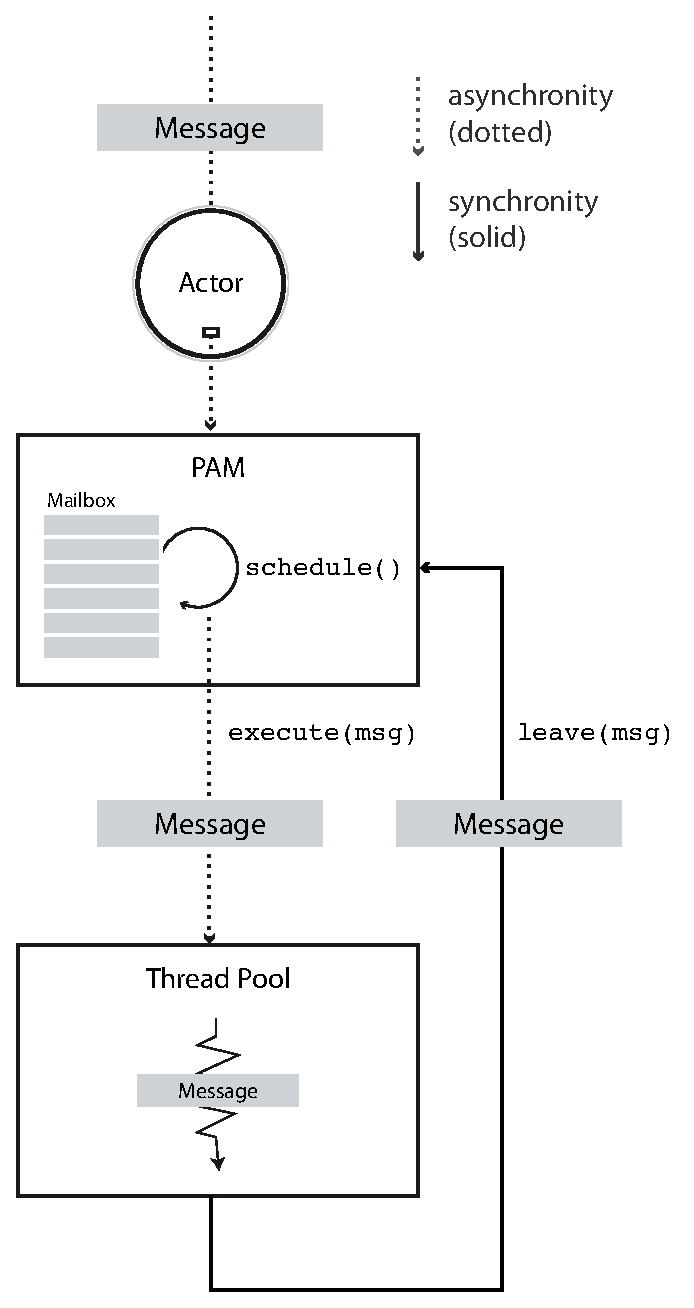
\includegraphics[width=6cm]{figures/pam_workflow-02.eps}
	\begin{caption}
		{The workflow of a PAM as proposed by Scholliers~et~al.~\cite{Scholliers2010a}} \label{fig:pamworkflow}
	\end{caption}
\end{figure}

\begin{enumerate}[\IEEEsetlabelwidth{6}]
	\item Incoming messages are handed over to PAM.
	\item PAM queue messages in a mailbox until the scheduling procedure runs.
	\item The messages matching the strategy are scheduled for execution. They are assigned to a thread out of the thread pool of the runtime. While the messages are processed, the code executed in the thread has free access to the actor's state.
	\item After completion of the execution, the thread which executed that task runs the \ct{leave} callback method of the monitor and PAM schedules remaining messages (if the queue is not empty).\\
\end{enumerate}

\subsection{Consequences and application}\label{sec:pamconsequencesandapplication}
On one hand, the injection of PAM leaves the initial actor-specific code untouched, what makes it modular and reusable. On the other hand, the workflow unveils a relaxation of the model: the encapsulation of an actor and its thread environment is broken during the execution of the message. This reintroduces possible concurrency issues such as data races that need to be explicitly avoided by the implemented scheduling policy. During scheduling however, known techniques for identifying errorneous behavior or a flaw in the implemented scheduling strategy, such as Datarace Detection~\cite{Cheng98a, Choi:2002:EPD:543552.512560} were not used. \autoref{fig:pamexecution} shows the positive impact of the exploited thread-parallelism with a multiple readers, single writer scheduler. The read accesses can be immediately executed in parallel reducing the total execution time. The write message is processed under mutual exclusion, depicted in the red area. As long as we are accessing only two different rows the performance is similar to the data partitioned actor in \autoref{fig:partitionedprocessing} indicated by the brown line. As soon as the actor is required to access more disjoint rows the overhead of data partitioning would grow. If the strategy could distinguish between the accessed rows, the reads after the write stage could also happen in parallel since they access a different row.

\begin{figure}[!htbp]
\centering
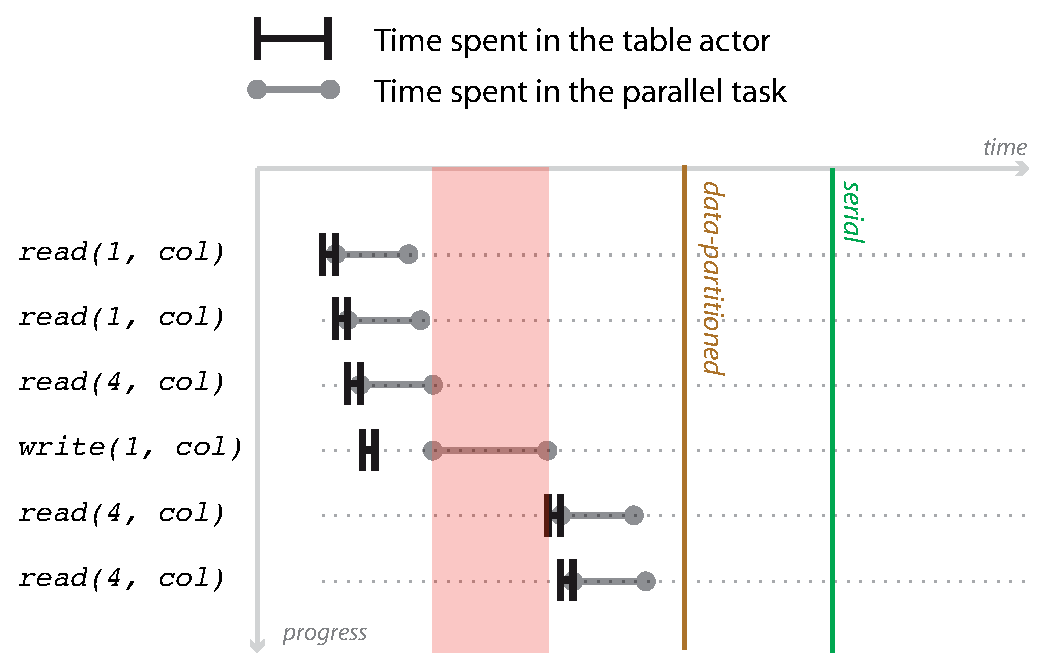
\includegraphics[width=\columnwidth]{figures/processing-03.eps}
\begin{caption}
	{The example processing powered by a PAM where the red area indicates the mutual exclusion. All the read accesses happen in parallel.} \label{fig:pamexecution}
\end{caption}
\end{figure}

\section{The Unified Model}\label{sec:unifiedmodel}
An alternative approach for exploiting parallelism was proposed by Imam and Sarkar~\cite{Imam:2012:ITP:2384616.2384671}. The authors integrated the divide-and-conquer strategy of the Async-Finish Model (AFM) into actor-based environments, namely Scala and Habanero Java. The combination of the AFM and the AM is called the Unified Model (UM). Furthermore, they introduced several enhancements to the AFM itself, for the purpose of circumventing some of its identified limitations.

\subsection{The Async Finish Model (AFM)}\label{subsec:afm}
The Async-Finish Model allows the creation (fork) and the joining of lightweight parallel tasks. To facilitate language integration, the authors provide corresponding language constructs, named \ct{async} and \ct{finish}. Tasks created in an \ct{async} block can be wrapped into a common \ct{finish} scope (join), having arbitrary levels of nesting. All tasks are enclosed into an unique dynamic Immediately Enclosing Finish (IEF). An IEF ensures that all forked processes terminate until program execution proceeds. The IEF can be explicitly created or is implicitly given for the entire program. Similar to PAM, the provided thread allocation is handled by the runtime. The Async-Finish Model works best if used with deterministic algorithms, ensures determinism in the absence of data races but is unable to handle non-determinism~\cite{Imam:2012:ITP:2384616.2384671}. Imam et al. state Quicksort as an example where the AFM is not able to exploit the non-deterministic availability of the sorted fragments and i.e. do computations on early available results. 

\subsection{Data-Driven Futures}\label{subsec:ddf}
The proposed AFM implementations permit the usage of Data Driven Futures (DDFs) in combination with an additional language construct, called \ct{asyncAwait}. A DDF is construct served by a producer (thread that does the computation) and awaited by a consumer (thread that awaits the result of the computation) and consists of three main callbacks:
\begin{itemize}
	\item \ct{put(value)} is invoked upon successful completion of the computation by the producer. Once a value is put into the future, the object gets hardened (becomes immutable) and the waiting consumer gets notified by the runtime.
	\item \ct{await()} is invoked by the \ct{asyncAwait} and the consumer is delayed by the runtime until a value was put into the DDF by the producer.
	\item \ct{get()} can be invoked by the consumer after awaiting the DDF. The previous waiting guarantees there was a put before and the DDF is associated by a value.
\end{itemize}
A parent task is capable of asynchronously awaiting the termination of an arbitrary number of subtasks (each represented through a DDF) without blocking the program execution. The combination of the async-finish constructs with DDFs introduces the possibility for parallelization inside the message-processing body (MBP)~\cite{Imam:2012:ITP:2384616.2384671}. DDFs are a suitable replacement for constructs like count-down latches (which represent shared state) to model join behavior. The presence of a blocking, enclosing finishing scope (multiple scopes are executed serially), prevents data races as well as avoids parallel execution of messages.

\subsection{Scope escaping and the paused state}\label{subsec:excapingandpausing}
As stated by Imam et al.~\cite{Imam:2012:ITP:2384616.2384671}, the enclosure of the processing of a message into a single finishing scope leads to serial execution of messages. To circumvent this limitation, the authors implemented the functionality to escape an actors own finishing scope. Escaping permits an actor to return immediately to the initial control flow without awaiting the termination of the spawned tasks inside the scope. The possibility to escape a scope is thought to be used only if the message does not require the internal state to be mutated. Nevertheless, the constraint of not mutating the actors state is neither monitored nor ensured, what enables potential data races.\\ 
To ensure the mutually-exclusive processing of critical sections emerging if multiple tasks run in parallel, an actor is able to be paused (by a \ct{pause} method). When an actor in paused state, it stops the processing of messages in the mailbox. To resume the actor from a paused state, the awaited task is required to invoke the \ct{resume} method explicitly upon termination.

\subsection{Consequences and application}\label{sec:umconsequencesandapplication}
On one hand, the capacity to escape the finishing scope enables the Unified Model to spawn tasks that process messages in parallel. In addition to being able to escape the finishing scope of an actor it is possible to exploit parallelism within the spawned task (intra-task parallelism). Critical sections (tasks that modify the actors state) can be protected by pausing the actor what prevents him from spawning new, concurrent tasks. On the other hand, escaping the scope reintroduces shared access to the actor's state and possible data races, which violates then fundamental guarantees provided by the Actor Model. As elaborated previously also for PAM, the occurrence of data races is not monitored or reported. Imam et al. indicated that they plan to investigate the integration of Dynamic Datarace Detection for future work. Dynamic Datarace Detection would enable the runtime to react to data races and e.g. reschedule erroneous messages. \autoref{fig:readerwriterum} demonstrates the behavior of the previously introduced table actor. \autoref{fig:parallelsearchum} provides an insight on the ways DDFs can be used to read from multiple rows.

\begin{figure}[!htbp]
\centering
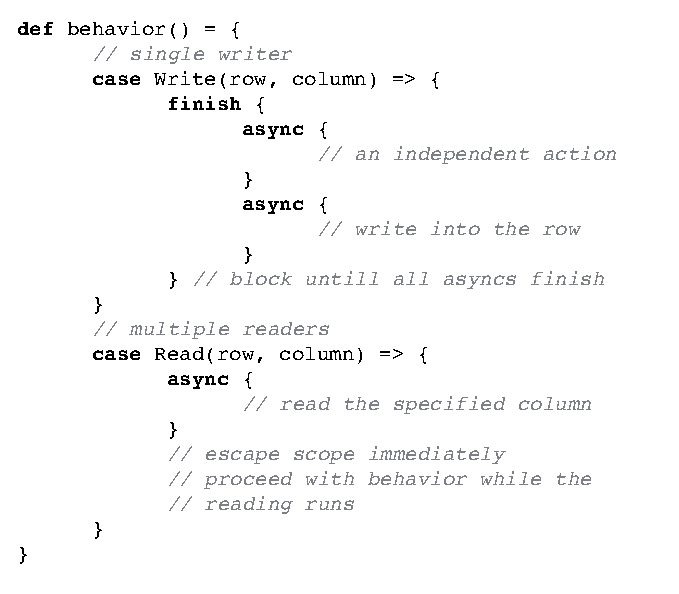
\includegraphics[width=\columnwidth]{figures/reader_writer_um-01.eps}
\begin{caption}
	{Skeleton of a reader-writer implementation in the UM in Scala. The behavior method is dedicated to implement the message handling of the actor.} \label{fig:readerwriterum}
\end{caption}
\end{figure}

\begin{figure}[!htbp]
\centering
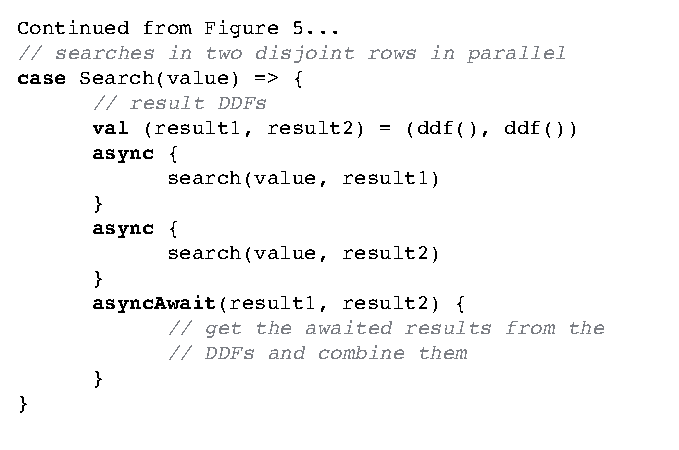
\includegraphics[width=\columnwidth]{figures/parallelsearchum-02.eps}
\begin{caption}
	{The skeleton of a fork-join search in a table actor, implemented exploiting the benefits of the Unified Model in Scala. Spawned tasks (async) are not explicitly embraced in a finishing scope, providing the possibility to execute searches in parallel.} \label{fig:parallelsearchum}
\end{caption}
\end{figure}

Even the rudimentary example in \figref{readerwriterum} suffers from possible data races. In reality the example does not fully exhibit intra-task parallelism and processing would be the same as in \autoref{fig:pamexecution}. Assuming we could establish intra-task parallelism in the write operation, we would arrive at a timeline, depicted in \autoref{fig:umexecution}.

\begin{figure}[!htbp]
\centering
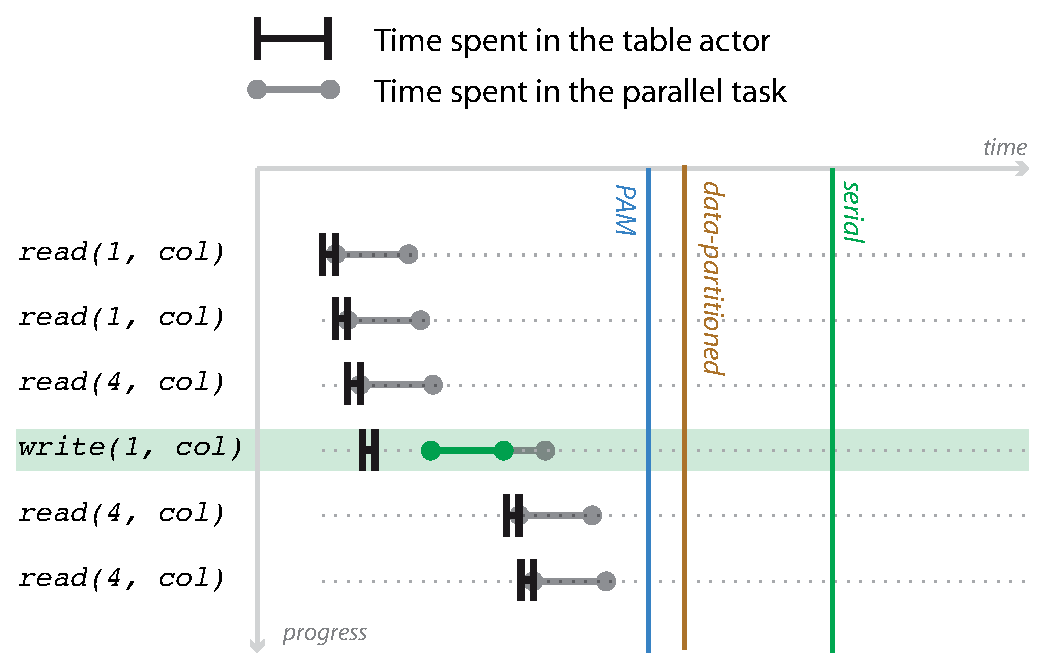
\includegraphics[width=\columnwidth]{figures/processing-04.eps}
\begin{caption}
	{An example processing sequence where we assume that the write stage benefits from intra-task parallelism and is executed faster.} \label{fig:umexecution}
\end{caption}
\end{figure}

\section{Comparison}\label{sec:comparison}
Consider a brief overview of the characteristics of the AM, PAM and the UM, provided in \autoref{tab:comparison}. The Actor Model is able to establish improved parallel processing of messages by data partitioning, suffering from data copying overheads. Parallel Actor Monitors as well as the Unified Model enable Actor Model implementations to process messages in parallel and improve scalability (as stated in a number of benchmarks \cite{Scholliers2010a, Imam:2012:ITP:2384616.2384671}) at the cost of data races and a certain loss of abstraction. While thread allocation and coordination is handled transparently for the programmer, the proposed mechanisms neither ensure the absence of data races, nor provide the capacity to detect data races. The concrete implementation of both approaches has to explicitly handle arising concurrency issues what can lead to additional complexity. PAM offer the capabilities to exploit enhanced parallelism without altering already existing Actor source code. The UM, on the other hand, requires rewriting existing Actor-specific code, but provides convenient mechanisms to implement fork-join functionality and exploit intra-task parallelism.

\begin{table}[!htbp]
	\centering
	\captionof{table}{Comparison of the approaches} \label{tab:comparison}
	
	\begin{tabularx}{\columnwidth}{ p{.35\columnwidth} *{3}{X}}
		\toprule
		& \bf{AM} & \bf{PAM} & \bf{UM} \\
		\hline
		task parallelism 	& \Bull	& \checkmark & \checkmark \\
		intra-task parallelism & \Bull & \X & \checkmark \\
		\hline
		Advantages & data race free & modular & fork-join\\
		& abstract & & parallelism\\
		\hline
		Disadvantages & scalability & \multicolumn{2}{c}{no encapsulation guarantee}\\
		& & \multicolumn{2}{c}{data races}\\
		& & \multicolumn{2}{c}{complexity}\\
		\bottomrule
	\end{tabularx}\bigskip
	\caption*{\centering \checkmark supportet, \Bull partially supported, \X not supported}
\end{table}

% C O N C L U S I O N
% % % % % % % % % % % % % % % % % % % % % % % % % % % % % % % % % %
\section{Conclusion}\label{sec:conclusion}
While both, PAM and the UM, exploit intra-actor parallelism and solve their respective objectives, they reintroduce possible data races. The handling, as well as detection and avoidance of data races has to be managed at a low level of the concrete implementation, which contradicts with the abstraction the Actor Model offers. As both approaches are relatively recent, further improvements on the presented approaches or different ways of exploiting intra-actor parallelism are very likely to be developed. One example could be the implementation of reliable mechanisms such as Dynamic Datarace Detection, for monitoring data races.

% A C K N O W L E D G M E N T S 
% % % % % % % % % % % % % % % % % % % % % % % % % % % % % % % % % %
\section*{Acknowledgments}
I'd like to thank Yarco Hayduk for his patience and the frequent reviews of my work.

% bibliography
% % % % % % % % % % % % % % % % % % % % % % % % % % % % % % % % %
\bibliographystyle{IEEEtran}
\bibliography{IEEEfull,bib/actor_model_survey}
\end{document}
